\documentclass[paper=a4,fontsize=12pt]{scrartcl}
\usepackage{geometry}
\usepackage{graphicx}
\geometry{verbose, a4paper, tmargin=25mm, bmargin=25mm, lmargin=25mm, rmargin=25mm}

\usepackage[utf8]{inputenc}
\usepackage[ngerman]{babel}

\usepackage{amsmath}

\usepackage{listings}
\usepackage{color}

\definecolor{mygreen}{rgb}{0,0.6,0}
\definecolor{mygray}{rgb}{0.5,0.5,0.5}
\definecolor{mymauve}{rgb}{0.58,0,0.82}

\lstset{ %
  backgroundcolor=\color{white},   % choose the background color; you must add \usepackage{color} or \usepackage{xcolor}
  basicstyle=\footnotesize,        % the size of the fonts that are used for the code
  breakatwhitespace=false,         % sets if automatic breaks should only happen at whitespace
  breaklines=true,                 % sets automatic line breaking
  captionpos=b,                    % sets the caption-position to bottom
  commentstyle=\color{mygreen},    % comment style
  deletekeywords={...},            % if you want to delete keywords from the given language
  escapeinside={\%*}{*)},          % if you want to add LaTeX within your code
  extendedchars=true,              % lets you use non-ASCII characters; for 8-bits encodings only, does not work with UTF-8
  frame=single,                    % adds a frame around the code
  keepspaces=true,                 % keeps spaces in text, useful for keeping indentation of code (possibly needs columns=flexible)
  keywordstyle=\color{blue},       % keyword style
  language=Octave,                 % the language of the code
  morekeywords={*,...},            % if you want to add more keywords to the set
  %numbers=left,                    % where to put the line-numbers; possible values are (none, left, right)
  %numbersep=5pt,                   % how far the line-numbers are from the code
  % numberstyle=\tiny\color{mygray}, % the style that is used for the line-numbers
  % rulecolor=\color{black},         % if not set, the frame-color may be changed on line-breaks within not-black text (e.g. comments (green here))
  showspaces=false,                % show spaces everywhere adding particular underscores; it overrides 'showstringspaces'
  showstringspaces=false,          % underline spaces within strings only
  showtabs=false,                  % show tabs within strings adding particular underscores
  stepnumber=2,                    % the step between two line-numbers. If it's 1, each line will be numbered
  stringstyle=\color{mymauve},     % string literal style
  tabsize=2,                       % sets default tabsize to 2 spaces
  title=\lstname                   % show the filename of files included with \lstinputlisting; also try caption instead of title
} 

% Grafiken einbinden 
\usepackage{graphicx}
\usepackage{here} % http://overspice.blogspot.ch/2007/10/latex-bilder-richtig-plazieren.html

\usepackage{fancyhdr} %Paket laden
\pagestyle{fancy} %eigener Seitenstil
\fancyhf{} %alle Kopf- und Fu�zeilenfelder bereinigen
\fancyhead[L]{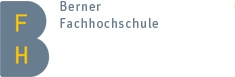
\includegraphics[width=3cm]{img/logo_bfh_de.jpg}} %Kopfzeile links
\fancyhead[C]{} %zentrierte Kopfzeile
\fancyhead[R]{Marco Berger, Andy Pollari} %Kopfzeile rechts
\renewcommand{\headrulewidth}{0.4pt} %obere Trennlinie
\fancyfoot[C]{\thepage} %Seitennummer
\renewcommand{\footrulewidth}{0.4pt} %untere Trennlinie

\makeatletter
\let\ps@plain\ps@fancy 
\makeatother


\usepackage{pgfplots}
\usepackage{filecontents}

\begin{filecontents*}{data.csv}
imgNames,width,height,megapixel,time
large-1.jpg,5184,3456,17.915904,0.0226542369937176
large-10.jpg,5184,3456,17.915904,0.02146350620254
large-2.jpg,5074,3383,17.165342,0.0214863869118607
large-4.jpg,5184,3456,17.915904,0.0218580817000087
large-5.jpg,5184,3456,17.915904,0.0217852369927837
large-6.jpg,5184,3456,17.915904,0.0220588715981288
large-7.jpg,11029,4695,51.781155,0.0621215927588625
large-8.jpg,5530,4142,22.90526,0.0278047313571249
large-9.jpg,3456,5184,17.915904,0.0213010064710382
medium-1.jpg,3000,2000,6,0.00726112305992598
medium-10.jpg,3000,2000,6,0.00749226491938986
medium-2.jpg,3000,2000,6,0.00722563461281637
medium-3.jpg,4085,2000,8.17,0.0102907157552829
medium-4.jpg,3000,2000,6,0.00744230092148555
medium-5.jpg,3000,2000,6,0.00724011016361108
medium-6.jpg,3000,2000,6,0.00741755239915911
medium-7.jpg,4698,2000,9.396,0.0112199527256528
medium-8.jpg,2670,2000,5.34,0.00675494573536265
medium-9.jpg,1333,2000,2.666,0.0035222283756284
small-1.jpg,1536,1024,1.572864,0.00216059269442299
small-10.jpg,1536,1024,1.572864,0.00209195056646099
small-2.jpg,1536,1024,1.572864,0.00207794196891772
small-3.jpg,2091,1024,2.141184,0.00275035465099447
small-4.jpg,1536,1024,1.572864,0.00213724503185088
small-5.jpg,1536,1024,1.572864,0.00212697206031915
small-6.jpg,1536,1024,1.572864,0.00201490327997303
small-7.jpg,2405,1024,2.46272,0.00306788286197516
small-8.jpg,1367,1024,1.399808,0.00195560021703987
small-9.jpg,683,1024,0.699392,0.00102636324666992
\end{filecontents*}

\begin{filecontents*}{performance-asymmetric-enc.csv}
imgName,width,height,megapixel,time
a.jpg,1536,1024,1.572864,2.76022765106889
large-1.jpg,5184,3456,17.915904,116.136913308893
large-10.jpg,5184,3456,17.915904,89.4094978200094
large-2.jpg,5074,3383,17.165342,44.2005362538717
large-4.jpg,5184,3456,17.915904,161.494887516968
large-5.jpg,5184,3456,17.915904,118.943474340458
large-6.jpg,5184,3456,17.915904,4.03735565763244
large-7.jpg,11029,4695,51.781155,368.004891378706
large-8.jpg,5530,4142,22.90526,3.99097091182303
large-9.jpg,3456,5184,17.915904,21.3691685776898
medium-1.jpg,3000,2000,6,1.53960242313531
medium-10.jpg,3000,2000,6,4.49044488431831
medium-2.jpg,3000,2000,6,2.92113276392549
medium-3.jpg,4085,2000,8.17,44.8644539423578
medium-4.jpg,3000,2000,6,23.7438710674599
medium-5.jpg,3000,2000,6,35.2777331833466
medium-6.jpg,3000,2000,6,5.08329352521547
medium-7.jpg,4698,2000,9.396,80.8788735866951
medium-8.jpg,2670,2000,5.34,69.5114117382816
medium-9.jpg,1333,2000,2.666,16.7334546488644
small-1.jpg,1536,1024,1.572864,3.20237186338881
small-10.jpg,1536,1024,1.572864,1.4994557611569
small-2.jpg,1536,1024,1.572864,13.1459755510447
small-3.jpg,2091,1024,2.141184,13.1007502604455
small-4.jpg,1536,1024,1.572864,15.2949816555788
small-5.jpg,1536,1024,1.572864,11.3610780738755
small-6.jpg,1536,1024,1.572864,1.66316448620911
small-7.jpg,2405,1024,2.46272,10.3404488301083
small-8.jpg,1367,1024,1.399808,0.429924871224825
small-9.jpg,683,1024,0.699392,4.74592661390982
\end{filecontents*}


\begin{document}
\thispagestyle{empty}
\newcommand{\Rule}{\rule{\textwidth}{1mm}}
\begin{center}
\Rule\vspace{5mm}
\sffamily\bfseries\Huge
Bildverschlüsselung mit Matlab
\vspace{1mm}\Rule
\vfill
\LARGE Bericht
\vfill
\Large Berger Marco \par
\Large Pollari Andy \par
\Large Programmierung in Matlab/Octave\par
\vfill
% \raisebox{7mm}{Universität}
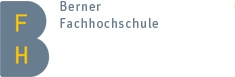
\includegraphics[height=16mm]{img/logo_bfh_de.jpg}
% \raisebox{7mm}{Osnabrück}\par
\vfill
\today
\end{center}
\newpage


\section{Einleitung}
In dieser Arbeit befassen wir uns mit der Anwendung verschiedener Verschlüsselungsalgorithmen
angewandt auf Bilder implementiert in Matlab. \\
Es ist zu erwähnen, dass es grundsätzlich zwei verschiedene Verschlüsselungsverfahren gibt:
\begin{itemize}
  \item Die symmetrische Verschlüsselung 
  \item Die asymmetrische Verschlüsselung 
\end{itemize}
Bei der symmetrischen Verschlüsselung wird mit einem Schlüssel verschlüsselt und mit demselben auch wieder entschlüsselt.
Bei der asymmetrischen Verchlüsselung hingegen gibt es zwei verschiedene Schlüssel: Einen öffentlichen Schlüssel zum verschlüsseln
und einen privaten Schlüssel zum entschlüsseln. \\ \\
Es gibt verschiedene asymmetrische Verschlüsselungsverfahren wie RSA, Merkle-Hellmann, RSA, \ldots \\
Auch bei den symetrischen Verschlüsselungsverfahren gibt es verschiedene wie DES, AES, One-Time-Pad, \ldots \\
Im Rahmen dieser Arbeit konzentrieren wir uns bei der symmetrische Verschlüsselung auf das \textit{One-Time-Pad} 
und bei den asymmetrisch Verschlüsselungsverfahren auf RSA. \\ \\
In dieser Arbeit haben wir festgestellt, dass sich Matlab nur bedingt eignet, um Bilder zu Verschlüsseln.
Für die symmetrische Verschlüsselung stiessen wir auf keine grösseren Probleme. Bei der asymmetrischen Verschlüsselung
trafen wir auf ein grösseres Problem bezüglich Primzahlen. Dieses Problem erläutern wir später im Kapitel \ref{results} \textit{Ergebnisse, Resultate}

\newpage 
\section{Grundlagen} 
In dieser Arbeit beschränken wir uns auf folgende Verschlüsselungsverfahren:
\begin{itemize}
  \item One Time Pad, als symmetrische Verschlüsselung
  \item Rivest, Shamir und Adleman (RSA), als asymmetrische Verschlüsselung.
\end{itemize} 
Daher beschränken wir uns ausschliesslich auf diese beiden Verfahren. 

\subsection{One-Time-Pad}
Beim One-Time-Pad haben wir einen Keystream der aus random Bits besteht.
Dieser Keystream muss mindestens so viele Bits lang sein, wie die zu verschlüsselnde Nachricht selbst.
In unserem Projekt ist die zu verschlüsselnde Nachricht ein JPG-Bild. \\
Die Idee beim One-Time-Pad ist, dass der Keystream nur einmal zum ver- respektive entschlüsseln verwendet wird. \\ \\
Die Verschlüsselung beim One-Time-Pad wird realisiert, 
indem das Bit an der Position $i$ des Bildes $m$ mit dem $i$-ten Bit des Keystreams $r$ XOR verknüpft wird.
% \begin{itemize}
%   \item Plaintext: $m = m_1 || m_2 || \cdots || m_k$
%   \item Ciphertext: $c = c_1 || c_2 | \cdots || c_k$
%   \item Keystream: $r = r_1 || r_2 | \cdots || r_k$
% \end{itemize}

\begin{figure}[H] 
	\centering
	\makebox[\textwidth]{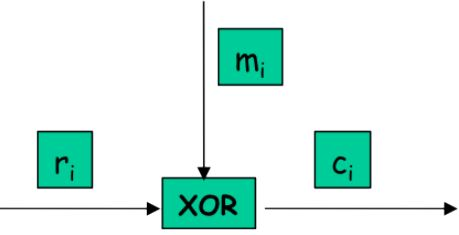
\includegraphics[width=7cm]{img/one-time-pad_enc.jpg}}
	\caption[One Time Pad Encryption]{One-Time-Pad Encryption}  
	\label{One-Time-Pad Encryption}  
\end{figure}
\begin{figure}[H] 
	\centering
	\makebox[\textwidth]{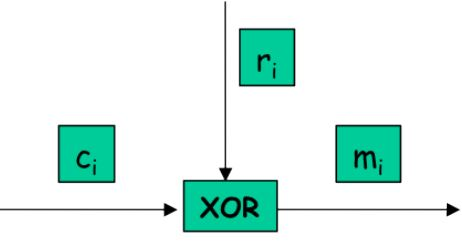
\includegraphics[width=7cm]{img/one-time-pad_dec.jpg}}
	\caption[One Time Pad Decryption]{One-Time-Pad Decryption}  
	\label{One-Time-Pad-enc} 
\end{figure}


\subsection{Rivest, Shamir und Adleman (RSA)} \label{RSA-intro}
RSA ist ein asymmetrisches kryptographisches Verfahren. Es wird zur Verschlüsselung aber auch für digitalen Signaturen verwendet.
In dieser Arbeit befassen wir uns ausschliesslich mit dem Verschlüsselungsverfahren von RSA.
\\ \\
RSA verwendet ein Schlüsselpaar bestehend aus einen privaten Schlüssel (Private Key) und einem öffentlichen Schlüssel  (Public Key).
Den Private Key verwendet man dabei um Daten zu entschlüsseln, die mit dem Public Key verschlüsselt worden sind. 

\subsubsection{Schlüssel Generierung}
Der Public Key ist ein Zahlenpaar $(e,N)$, und der Private Key ist auch ein Zahlenpaar $(d,N)$.
$e$ des Public Keys wird auch den Verschlüsselungsexponenten genannt.
$d$ des Private Keys wird auch den Entschlüsselungsexponenten genannt. 
Bei beiden Zahlenpaaren ist N gleich und wird \textit{RSA Modul} genannt.
Eine kurze grobe Beschreibung, wie die oben genannten Schlüssel generiert werden:
\begin{itemize}
  \item Die Primzahlen $p$ und $q$ zufällig wählen, $p \neq q$
  \item Den RSA-Modul $N$ berechnen \begin{align} N = p \cdot q \end{align}
  \item $\varphi(N)$ berechnen \begin{align} \varphi(N) = (p-1) \cdot (q-1)\end{align}
  \item $e$ wählen, welches teilerfremd von $\varphi(N)$ ist
  \item $d$ wählen, wobei gilt \begin{align} e \cdot d \equiv_N mod \varphi(N)\end{align} $d$ ist also das multiplikativ Inverse Element von $e$ im Bezug auf $\varphi(N)$
\end{itemize}

\subsubsection{Verschlüsselung / Entschlüsselung}
Möchten wir eine Nachricht $m$ verschlüsseln, so wird die Nachricht $m$ mit dem Verschlüsselungsexponenten $e$ potenziert.
Man erhält so den Ciphertext $c$ (Geheimtext).
\begin{align}
	c \equiv_N m^e
\end{align}

Um den Ciphertext $c$ zu entschlüsseln, muss $c$ mit dem Entschlüsselungsexponenten $d$ potenziert werden.
So erhalten wir wieder die Ursprungsnachricht $m$.
\begin{align}
	m \equiv_N c^d
\end{align}

 

\newpage
\section{Vorgehen, Methoden Analysen}
Da wir die Grundlagen der zu verwendenden Verschlüsselungen bereits durch unsere Studium-Vertiefung IT-Security hatten,
konnten wir uns schnell der Implementierung widmen.

\subsection{Implementierung der symmetrischen Verschlüsselung}
Wie bereits erwähnt haben wir uns für eine One Time Pad Verschlüsselung entschieden.
Dabei wird ein Bild in eine Matrix $M_M$ gelesen. 
Für das One Time Pad erstellen daraufhin eine Matrix $M_R$ mit Zufallswerten und exakt der Grösse, des eingelesenen Bildes.
Die beiden Matrizen werden XOR miteinander verknüpft, was eine neue Matrix $M_C$ ergibt und dem verschlüsselten Bild entspricht.
Nachträglich haben wir die Zeitmessung eingebaut, um Auswertungen machen zu können.


\subsection{Implementierung der asymmetrischen Verschlüsselung}
Bei der asymmetrischen Verschlüsselung haben wir uns für die RSA Verschlüsselung entschieden.
Die Implementiertung erfolgte erst ziemlich genau so, wie im Grundlagen Kapitel \ref{RSA-intro} beschrieben:
Erst die Schlüsselgenerierung und anschliessend wurde jeder Wert des Bildes mit den Bilder ver- und entschlüsselt.
Bei der RSA Implementierung stiessen wir auf einige Probleme, die wir im Kapitel \ref{problems-RSA} erläutern.
Nach der vollständigen Implementierung der Ver- resp. Entschlüsselung, wurden auch hier noch Zeitmessungen eingebaut, um Auswertungen
machen zu können.

\newpage
\section{Ergebnisse, Resultate} \label{results} 

\subsection{Symmetrische Verschlüsselung}
\subsubsection{Performance bei der symmetrischen Verschlüsselung}
\begin{tikzpicture}
\begin{axis}[width=\textwidth, height=0.6\textwidth,
		title={Performance - Symmetrische Verschlüsselung},
		ylabel={Megapixel},
		xlabel={Sekunden}
		]
\addplot table [x=time, y=megapixel, col sep=comma] {data.csv};
\end{axis}
\end{tikzpicture} \\
Unserer Meinung nach ist die Performance bei der symmetrischer Verschlüsselung sehr akzeptabel.
Die obere Grafik zeigt, dass die Verschlüsselungsdauer wie erwartet linear zur Anzahl Bildpunkten ist.
Um ein Bild von 50 Megapixel zu verschlüsseln braucht unser Matlab Programm 0.06s.
Die Verschlüsselungsdauer ist mit der Entschlüsselungsdauer identisch, da die gleichen Operationen (XOR) durchgeführt werden.
Bezüglich der Performance eignet sich Matlab unserer Meinung sehr gut für eine symmetrische Verschlüsselung mit dem One-Time-Pad.

\subsubsection{Wiedererkennbarkeit des Bildes}
Mehrere Versuche zeigten, dass das Originalbild nach der Verschlüsselung in keiner Weise wiedererkennbar ist.
Auch in diesem Punkt, überzeugt die symmetrische Verschlüsselung mit dem One-Time-Pad.
Die Abbildung \ref{sym-enc-result} zeigt ein Beispiel des Resultates.
\begin{figure}[H] 
	\centering
	\makebox[\textwidth]{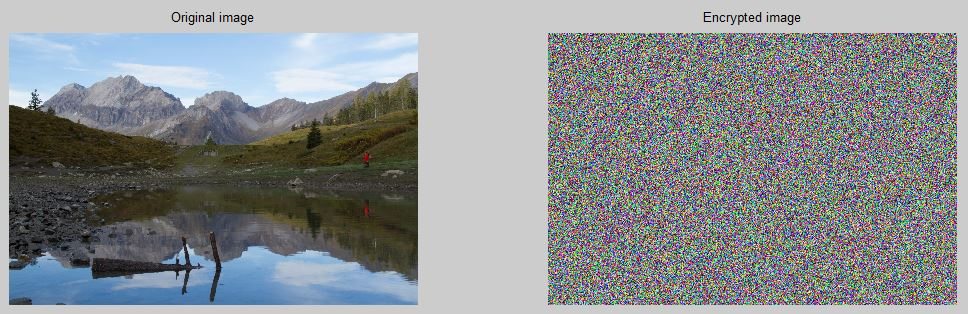
\includegraphics[width=\textwidth]{img/sym-enc-result.jpg}}
	\caption[One Time Pad - Verschlüsselung]{One Time Pad - Verschlüsselung}  
	\label{sym-enc-result} 
\end{figure}

\subsubsection{Verschlüsseltes Bild Speichern und anzeigen}
Das verschlüsselte Bild kann als valides JPG Bild abgespeichert werden und in einem
gewöhnlichen Bildbetrachtungsprogramm interpretiert werden.
 
\newpage
\subsection{Asymmetrische Verschlüsselung}
\subsubsection{Performance bei der asymmetrischen Verschlüsselung}
% \begin{tikzpicture}
% \begin{axis}[width=\textwidth, height=0.6\textwidth,
% 		title={Performance - Symmetrische Verschlüsselung},
% 		ylabel={Megapixel},
% 		xlabel={Sekunden}
% 		]
% \addplot table [x=time, y=megapixel, col sep=comma] {performance-asymmetric-enc.csv};
% \end{axis}
% \end{tikzpicture} \\
Bei der asymmetrischen Verschlüsselung lässt die Performance zu wünschen übrig.
Bei der Verschlüsselung eines 50 Megapixel zu verschlüsseln, brauchten wir auf unseren
Workstations durchschnittlich 337 Sekunden, also ~5.6 Minuten.
\subsubsection{Wiedererkennbarkeit des Bildes}
 Bei einigen Bildern konnte man beim verschlüsselten Bild noch Umrisse, Konturen oder grössere
 Flächen wiedererkennen.
 Somit wurden die Bilder nicht immer völlig verschleiert und teilweise waren sie wiedererkennbar.
 \begin{figure}[H] 
	\centering
	\makebox[\textwidth]{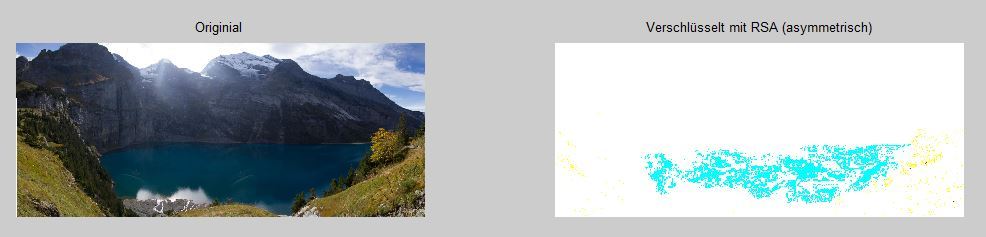
\includegraphics[width=\textwidth]{img/asym-enc-result.jpg}}
	\caption[RSA - Verschlüsselung]{RSA - Verschlüsselung}  
	\label{asym-enc-result} 
\end{figure}


\subsubsection{Problem bei der RSA Verschlüsselung} \label{problems-RSA}
\paragraph{Ungültiges Bild} \label{problem-white}
Wie man in der Abbildung \ref{asym-enc-result} sieht, ist der grösste Teil
des Bildes weiss.
Grund dafür ist, dass wir mit JPG Bilder von 8-Bit arbeiteten.
Mit einer Farbtiefe von 8-Bit kann man pro Farbe 255 verschiedene Werte darstellen.
der Bildes weiss.
Grund dafür ist, dass wir mit JPG Bildern von 8-Bit Farbtiefe arbeiteten.
Mit einer Farbtiefe von 8-Bit kann man pro Farbe 256 verschiedene Werte darstellen.

Da wir nun die RGB Werte von jedem Pixel verschlüsseln, kann es also für die einzelnen
RGB Werte grössere Farbwerte als 255 geben, was eigentlich zu Farben führt,
die ausserhalb des 8-Bit Spektrums liegen.

Der Bildbetrachter von Abbildung \ref{sym-enc-result} interpretiert diese double 
RGB-Werte nun als Weiss. 
Es gehen also nicht Informationen verloren, wie es vielleicht auf den ersten Blick schient,
sondern viele Werte liegen ausserhalb der 8-Bit Tiefe, welche dann weiss angezeigt werden.
Somit entstehen neu double-Werte die Matlab dennoch als Bild darstellen kann. Werte die nun 
ausserhalb der 8-Bit Farbtiefen liegen, werden als weiss interpretiert.
Matlab kann nun mit der RSA Modulo-Operation das Ausgangsbild wieder korrekt zurückrechnen. 
Allerdings ist es nicht möglich, dieses Bild direkt interpretierbar abzuspeichern 
(jedenfalls ohne zusätzliche mapping Operationen). 

Es wäre möglich, mit Bilder von einer höheren Farbtiefe zu arbeiten wie bspw. 16-Bit Bildern.
Das oben genannte Problem wäre somit immer noch bestehend, einfach erst mit grösseren Zahlen.


\paragraph{Problem Performance} Die Performance mit der RSA Verschlüsselung ist schlecht.
Im Allgemeinen eignet sich die asymmetrische Verschlüsselung nicht bei grossen Dateien.
Üblicherweise wird ein hybrides Verschlüsselungsverfahren verwendet indem
ein symmetrischer Schlüssel asymmetrisch verschlüsselt wird.
Auch unsere Performance Tests zeigten, dass die Performance bei der RSA-Verschlüsselung
sehr schlecht ist (rund 1000x langsamer) im Vergleich zu der symmetrischen Verschlüsselung.


\paragraph{Problem Pixel für Pixel Verschlüsselung} 
Jedes Pixel besteht aus drei Farben: Rot, Grün und Blau.
Bei unseren Tests haben wir nur mit JPG Bildern mit einer Farbtiefe von 8-Bit gearbeitet.
Das heisst dass wir für die Farben Rot, Grün, Blau je 255 verschiedene Mögliche Werte haben können.
Unser asymmetrisches Verschlüsselungsverfahren iteriert durch jedes Pixel $P_n$ und verschlüsselt
in Jedem Pixel die Farben.
\begin{align} 
Original: &P_n(R,G,B) \\
Encrypted: &P_n'(enc(R), enc(G), enc(B))
\end{align}
Durch das RSA Verschlüsselungsverfahren kann es dann aber für $enc(R|G|B)$ Werte geben die nicht mehr
im 8-Bit Bereich sind (Problem oben beschrieben).
Ein anderes Problem ist aber auch, dass der selbe RGB-Wert verschlüsselt auch immer den zum selben
verschlüsselten Wert führt. Dies erklärt auch die hellblaue Fläche im verschlüsselten Bild 
in der Abbildung \ref{asym-enc-result}

\paragraph{Keine grossen Primzahlen}
Wir wussten bereits im Vornhinein, dass wir für Matlab nur relativ kleine Primzahlen nutzen können.
Mit einer Bruteforce Attacke könnte man also unsere mit Matlab asymmetrisch verschlüsselten Bilder
in absehbarer Zeit "`entschlüsseln"'.
 
 
\newpage
\section{Ahnang}
\subsection{Code}
\subsubsection{Symmetrische Verschlüsselung}
\lstinputlisting[language=Matlab, title=matlab-enc-symetric.m]{../matlab/matlab-enc.m}
\lstinputlisting[language=Matlab, title=encData.m]{../matlab/encData.m}

\newpage
\subsubsection{Asymmetrische Verschlüsselung}
\lstinputlisting[language=Matlab, title=matlab-enc-assymetric.m]{../matlab/matlab-enc-assymetric.m}
\lstinputlisting[language=Matlab, title=encDataRSA.m]{../matlab/encDataRSA.m}

\end{document}
